\section{FUSE}
\label{sec:fuse}
\gls{FUSE} is a library that provides an interface to create filesystems in userspace rather than in kernel space which is otherwise often considered the standard when writing commercial filesystems\,\cite{Libfuse2021}. The reason to implement a filesystem in kernel space is that it leads to faster system calls than when writing a filesystem in userspace. However, while filesystems using \gls{FUSE} are generally slower than \mbox{kernel-based} filesystems, using \gls{FUSE} simplifies the process of creating filesystems.

macFUSE is a port of \gls{FUSE} that runs on Apple's macOS operating system and it extends the \gls{FUSE} \gls{API}\,\cite{HomeMacFUSE}. macFUSE provides an \gls{API} for C and Objective C.  As macFUSE is an extension of the \gls{FUSE} library, there is a possibility that it is easy to port the macFUSE filesystems to the normal \gls{FUSE} gls{API} and mount them on, for instance, a Linux operating system. However, information about this has not been found. No experiments have been conducted to see if filesystems developed using macFUSE can be mounted on \mbox{non-macOS} operating systems.

\Cref{fig:fuse_desc} presents an overview how \gls{FUSE} works. \gls{FUSE} consists of a kernel space part and a userspace part that perform different tasks\,\cite{vangoorFUSENotFUSE2017}. The kernel part of \gls{FUSE} operates with the \gls{VFS}, which is a layer in both the Linux kernel and the macOS kernel that exposes a filesystem interface for userspace applications\,\cite{goochOverviewLinuxVirtual, singhMacOSInternals2006}. The \gls{VFS} interface is independent of the underlying filesystem and is an abstraction of the underlying filesystem operations, which can be used on any filesystem the \gls{VFS} supports. The userspace part of \gls{FUSE} communicates with the kernel space part through a block device. Operations on a mounted \gls{FUSE} filesystem are sent to the \gls{VFS} from the user application, which are then sent to the kernel part of \gls{FUSE}. If needed, the operations are transmitted to the userspace part of \gls{FUSE} where the operation is handled, and a response is sent back to the \gls{VFS} and the user application through the \gls{FUSE} kernel module. However, some actions can be handled by the \gls{FUSE} kernel module directly, such as if the file is cached in the kernel part of \gls{FUSE}\,\cite{vangoorFUSENotFUSE2017}. The response is then sent back to the user application from the kernel module through the \gls{VFS}.

\begin{figure}[!ht]
	\begin{center}
	  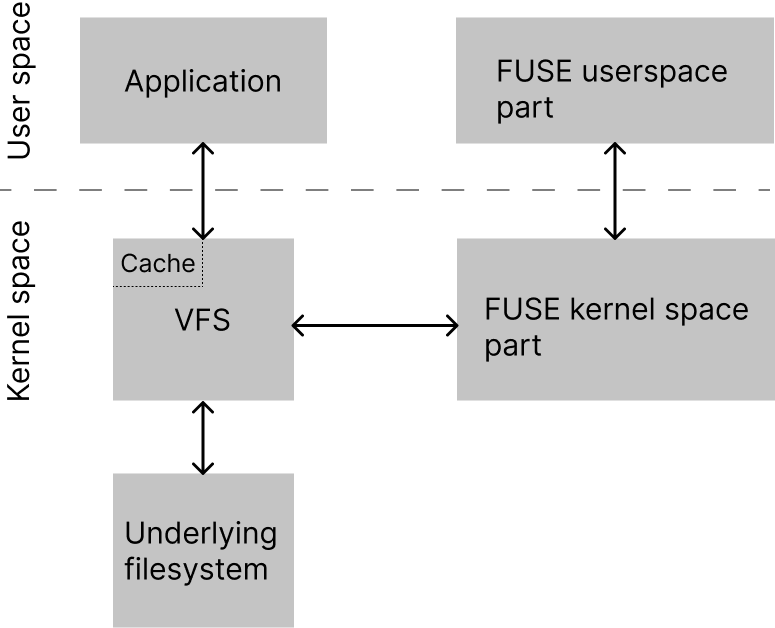
\includegraphics[width=0.75\textwidth]{figures.nosync/fuse_description.png}
	\end{center}
	\caption{Simple visualization of how \gls{FUSE} operations are executed}
	\label{fig:fuse_desc}
\end{figure}

Figure~\ref{fig:fuse_desc} also shows a kernel cache, also known as the \gls{UBC}\cite{Silvers2000}. The data stored in a macFUSE filesystem can be cached by the kernel to provide faster filesystem operations\,\cite{vangoorFUSENotFUSE2017, fleischerMountOptionsOsxfuse2020, gowdappaExperiencesFUSEReal2019}. This can be disabled, for instance, when the filesystem can be modified independently of filesystem operations on the computer, such as for a distributed filesystem where changes can be made by another user at any time.

\gls{FUSE} allows large files in the filesystems. The file operation offset, used to read or write at a byte location inside a file, is an unsigned 64-bit integer; thus, the filesystem operations can read and write to files as large as \SI{18}{\exbi\byte} bytes. 